\documentclass[11pt]{article}
\usepackage{apchem}
\doctitle{Unit 1 Content Guide}
\docsubtitle{A Comprehensive Review of Atomic Structure and Properties, Topics 1.1--1.8}
\docstatus{Study draft}
\begin{document}
\titleblock
\begin{abstract}
This guide covers all of Unit 1, Atomic Structure and Properties, in nine sections: one for each of Topics 1.1--1.8 in course order, plus a final section on lab skills and free-response technique. Each section gives the definitions, equations and particle-level reasoning the topic needs, at least one worked example, the phrasing that earns free-response points and the mistakes that cost them. The worked examples use their own numbers, so none of them give away an item in \emph{Unit 1 Practice Set A} or \emph{Unit 1 Practice Set B}; the answer keys of both sets point back to the section numbers here. Plan on about 60 minutes for a full read with a calculator out. Read a section, cover its worked examples and redo them on paper, and only then move on.
\end{abstract}
\leadline{Usage}{first pass, read Sections 1--9 in order and redo every worked example. Then take \emph{Unit 1 Practice Set A} cold; reread the section behind every miss, and take \emph{Unit 1 Practice Set B} two or three days later. The last page is a one-page summary for the night before the unit test. Unit 1 is 7--9\% of the AP multiple-choice section, but every later unit assumes it.}

\section{Moles and molar mass (Topic 1.1)}\label{t:1.1}
\subsection{The mole connects grams to particles}
Atoms are far too small to count one by one, so chemists count them in moles. One mole is $6.022\times10^{23}$ particles (Avogadro's number, $N_A$). The average mass of one atom in atomic mass units (amu) is numerically equal to the mass of one mole of those atoms in grams: one C atom averages 12.01 amu, and one mole of C atoms has a mass of 12.01 g. That is why the periodic table can be read in either unit.
\[ n = \frac{m}{M} \qquad N = n\,N_A \]
\begin{itemize}
\item $n$ is the amount in moles, $m$ the mass in grams, $M$ the molar mass in $\mathrm{g\,mol^{-1}}$, $N$ the number of particles.
\item Molar mass of a compound = sum of the atomic masses in its formula. For $\ce{Ca(NO3)2}$, the parentheses multiply everything inside: $40.08 + 2(14.01) + 6(16.00) = 164.10\unit{g\,mol^{-1}}$.
\item Be clear about which particle you are counting: molecules, formula units, atoms, or atoms of one element. One mole of $\ce{C3H8}$ contains 3 mol of C atoms, 8 mol of H atoms and 11 mol of atoms in all.
\end{itemize}

\worked{1.1} How many grams are in 0.150 mol of glucose, $\ce{C6H12O6}$? $M = 6(12.01) + 12(1.008) + 6(16.00) = 180.16\unit{g\,mol^{-1}}$, so $m = 0.150 \times 180.16 = 27.0\unit{g}$.

\worked{1.2} How many hydrogen atoms are in 11.0 g of propane, $\ce{C3H8}$ ($M = 44.09\unit{g\,mol^{-1}}$)? $n = 11.0/44.09 = 0.249\unit{mol}$ of molecules; $\times\,8 = 1.996\unit{mol}$ of H; $\times\,N_A = 1.20\times10^{24}$ H atoms.

\worked{1.3} A sample of a metal contains $1.81\times10^{23}$ atoms and has a mass of 7.07 g. $n = 1.81\times10^{23}/6.022\times10^{23} = 0.301\unit{mol}$, and $M = 7.07/0.301 = 23.5\unit{g\,mol^{-1}}$, closest to sodium (22.99).

\errorsh
\begin{itemize}
\item Dividing when you should multiply. Write the units and let them cancel: $\mathrm{g} \times \mathrm{mol/g}$ gives mol.
\item Counting molecules when the question asks for atoms (or the reverse).
\item Forgetting the subscript outside parentheses: $\ce{Ca(NO3)2}$ has 6 oxygen atoms, not 3.
\end{itemize}

\section{Mass spectra of elements (Topic 1.2)}\label{t:1.2}
\subsection{What a mass spectrum shows}
Most elements occur as a mixture of \emph{isotopes}: atoms with the same number of protons but different numbers of neutrons, and so different masses. A mass spectrometer ionizes the atoms and separates them by mass (strictly, by mass-to-charge ratio). For an element, each isotope gives one peak: its position is the isotope's mass and its height is the isotope's relative abundance.

\begin{center}
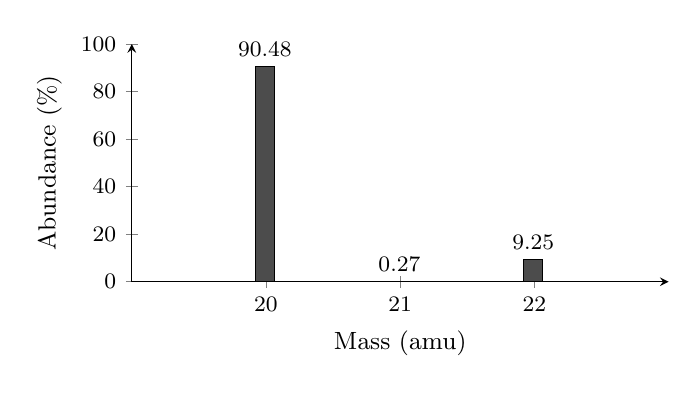
\begin{tikzpicture}
\begin{axis}[width=8.4cm,height=4.6cm,ybar,bar width=7pt,xmin=19,xmax=23,ymin=0,ymax=100,
  xlabel={Mass (amu)},ylabel={Abundance (\%)},xtick={20,21,22},axis lines=left,
  nodes near coords,every node near coord/.append style={font=\footnotesize},
  tick label style={font=\footnotesize},label style={font=\small}]
\addplot[fill=black!70,draw=black] coordinates {(19.992,90.48) (20.994,0.27) (21.991,9.25)};
\end{axis}
\end{tikzpicture}

{\small\itshape Mass spectrum of neon: three isotopes, Ne-20 dominant.}
\end{center}

\subsection{Average atomic mass}
The atomic mass on the periodic table is the abundance-weighted average of the isotope masses:
\[ \text{average atomic mass} = \sum (\text{isotope mass}) \times (\text{fractional abundance}). \]
The average always lies between the lightest and the heaviest isotope, and it sits closer to the most abundant one. This is why atomic masses are not whole numbers even though every atom has a whole number of protons and neutrons.

\worked{2.1} Neon (spectrum above): $19.992(0.9048) + 20.994(0.0027) + 21.991(0.0925) = 18.089 + 0.057 + 2.034 = 20.18$ amu, matching the periodic table.

\worked{2.2} An element has two isotopes, of mass 106.905 and 108.905 amu, and an average atomic mass of 107.87 amu. Let $x$ be the fraction of the lighter isotope: $106.905x + 108.905(1-x) = 107.87$, so $2.000x = 1.035$ and $x = 0.518$: 51.8\% and 48.2\% (silver).

\subsection{Molecules in a mass spectrum}
A diatomic molecule of an element with two isotopes can combine them in three ways. For bromine (about 50.7\% Br-79 and 49.3\% Br-81), intact $\ce{Br2}$ gives peaks at 158, 160 and 162 amu in a ratio close to $1:2:1$, because the mixed pair can form two ways (79--81 or 81--79).

\errorsh
\begin{itemize}
\item Taking the simple mean of the isotope masses. Weight each one by its abundance.
\item Reporting the most abundant isotope's mass as the atomic mass.
\item Saying isotopes behave differently in reactions. They have the same electron configuration, so their chemistry is the same.
\end{itemize}

\section{Elemental composition of pure substances (Topic 1.3)}\label{t:1.3}
\subsection{Law of definite proportions}
A pure compound always contains the same elements in the same proportion by mass, whatever its source or the size of the sample. Water is always 11.2\% H and 88.8\% O by mass. Any sample of a pure compound therefore has a fixed mass percent of each element:
\[ \text{mass \% of element} = \frac{(\text{atoms of the element per formula}) \times (\text{atomic mass})}{\text{molar mass}} \times 100\%. \]

\subsection{Empirical and molecular formulas}
The \emph{empirical formula} is the simplest whole-number mole ratio of the atoms. The \emph{molecular formula} is a whole-number multiple of it: glucose $\ce{C6H12O6}$ has empirical formula $\ce{CH2O}$. Ionic compounds are always written as empirical formulas.

To find an empirical formula from mass data:
\begin{enumerate}
\item Take a 100 g sample if you are given percentages, so each percent becomes grams.
\item Convert each mass to moles.
\item Divide every mole value by the smallest one.
\item If a ratio ends in about .5, .33 or .25, multiply all of them by 2, 3 or 4 to reach whole numbers.
\end{enumerate}
To get the molecular formula, divide the molar mass by the empirical-formula mass and multiply the subscripts by that whole number.

\worked{3.1} A compound is 85.6\% C and 14.4\% H. Per 100 g: C $85.6/12.01 = 7.13$ mol; H $14.4/1.008 = 14.3$ mol. Ratio $1 : 2.00$: empirical formula $\ce{CH2}$. If its molar mass is 56 g/mol, then $56/14.03 = 4$ and the molecular formula is $\ce{C4H8}$.

\worked{3.2} A sample of iron oxide contains 2.79 g Fe and 1.20 g O. Fe: $2.79/55.85 = 0.0500$ mol; O: $1.20/16.00 = 0.0750$ mol. Ratio $1 : 1.5$; multiply by 2: $\ce{Fe2O3}$.

\worked{3.3} Mass percent of sulfur in $\ce{Al2(SO4)3}$ ($M = 342.17$): $3(32.07)/342.17 = 28.1\%$.

\subsection{Combustion analysis}
When a compound of C and H (and possibly O) burns completely, all of its carbon ends up in $\ce{CO2}$ and all of its hydrogen in $\ce{H2O}$. Moles of C = moles of $\ce{CO2}$; moles of H = $2 \times$ moles of $\ce{H2O}$. Any mass left over after C and H is oxygen.

\worked{3.4} Burning 0.300 g of a compound of C, H and O gives 0.440 g $\ce{CO2}$ and 0.180 g $\ce{H2O}$. C: $0.440/44.01 = 0.0100$ mol (0.120 g); H: $2(0.180/18.02) = 0.0200$ mol (0.0202 g); O: $0.300 - 0.120 - 0.020 = 0.160$ g $= 0.0100$ mol. Ratio $1:2:1$: $\ce{CH2O}$.

\errorsh
\begin{itemize}
\item Using mass percentages directly as subscripts. Convert to moles first.
\item Forgetting the 2 in $\ce{H2O}$ in combustion analysis.
\item Rounding 1.5 to 2 (or 1.33 to 1). Multiply through instead.
\end{itemize}

\section{Composition of mixtures (Topic 1.4)}\label{t:1.4}
A \emph{mixture} contains two or more substances that are not chemically combined, in proportions that can vary. Its elemental composition therefore varies too, and it always lies between the compositions of its pure components. Two diagnostic ideas:
\begin{itemize}
\item If different samples of a material have different mass percents of an element, the material is a mixture.
\item If a measured mass percent is outside the range of any proposed pure components, the proposed composition is wrong: an impurity with more (or less) of that element must be present.
\end{itemize}
To find how much of a component is in a mixture, use a property that only that component has: a mass of an element only it contains, or a gas only it releases.

\worked{4.1} A 5.00 g mixture of $\ce{NaHCO3}$ and NaCl is analyzed and found to contain 0.680 g of carbon. Only $\ce{NaHCO3}$ (84.01 g/mol) contains carbon, one C per formula. Moles of $\ce{NaHCO3}$ = $0.680/12.01 = 0.0566$; mass $= 0.0566 \times 84.01 = 4.76$ g, so the mixture is $4.76/5.00 = 95.1\%$ $\ce{NaHCO3}$.

\worked{4.2} A copper ore is 22.0\% Cu by mass. Its only copper mineral is $\ce{CuFeS2}$ (34.6\% Cu). The mass percent of $\ce{CuFeS2}$ in the ore is $22.0/34.6 = 63.6\%$.

\errorsh
\begin{itemize}
\item Reporting the mass of the measured element (or gas) as the mass of the component.
\item Assuming a mixture is a compound because it ``looks uniform.'' Composition, not appearance, is the test.
\end{itemize}

\section{Atomic structure and electron configuration (Topic 1.5)}\label{t:1.5}
\subsection{Coulomb's law}
Every argument in this unit comes back to the attraction between the positive nucleus and the negative electrons:
\[ F \propto \frac{q_1 q_2}{r^2} \qquad\text{(potential energy } \propto q_1q_2/r\text{)}. \]
An electron is held more strongly when the nuclear charge it feels is larger or when it is closer to the nucleus. Inner (core) electrons \emph{shield} outer electrons from part of the nuclear charge, so valence electrons feel an \emph{effective} nuclear charge that is roughly (protons $-$ core electrons).

\subsection{Shells, subshells and the Aufbau order}
Electrons occupy shells ($n = 1, 2, 3, \dots$) split into subshells $s$ (2 electrons), $p$ (6), $d$ (10) and $f$ (14). In the ground state they fill in order of increasing energy:
\[ 1s\;2s\;2p\;3s\;3p\;4s\;3d\;4p\;5s\;4d\;5p\;\dots \]
\begin{itemize}
\item Noble-gas shorthand: Se is $[\ce{Ar}]\,4s^2 3d^{10} 4p^4$.
\item Within a subshell, electrons occupy separate orbitals before pairing (Hund's rule), and the two electrons in one orbital have opposite spins (Pauli principle).
\item Cations of transition metals lose their $4s$ electrons \emph{before} their $3d$ electrons: Zn is $[\ce{Ar}]\,4s^2 3d^{10}$ and $\ce{Zn^2+}$ is $[\ce{Ar}]\,3d^{10}$.
\item Anions add electrons to the next open subshell: $\ce{N^3-}$ is $1s^2 2s^2 2p^6$, the configuration of Ne.
\item An \emph{excited state} has an electron in a higher subshell while a lower one still has room, for example $1s^2 2s^1 2p^1$ for Be.
\end{itemize}
The AP exam does not test the exceptions (Cr, Cu and their relatives).

\worked{5.1} Ti ($Z = 22$): $[\ce{Ar}]\,4s^2 3d^2$. $\ce{Ti^2+}$: $[\ce{Ar}]\,3d^2$. $\ce{Ti^4+}$: $[\ce{Ar}]$, isoelectronic with Ar, $\ce{Cl-}$ and $\ce{Ca^2+}$.

\worked{5.2} Which feels the larger effective nuclear charge, a valence electron of Na or of Cl? Both are in $n = 3$ with 10 core electrons. Na: about $11 - 10 = +1$; Cl: about $17 - 10 = +7$. Cl's valence electrons are held far more strongly.

\frph Name both parts of Coulomb's law: ``more protons'' (or ``greater effective nuclear charge'') \emph{and} ``same shell / similar shielding'' or ``farther from the nucleus / more shielding.'' Answers that only say ``it wants a full octet'' or ``it is more stable'' earn nothing.

\section{Photoelectron spectroscopy (Topic 1.6)}\label{t:1.6}
In photoelectron spectroscopy (PES), high-energy photons knock electrons out of atoms, and the kinetic energy of each ejected electron is measured. The \emph{binding energy} is the energy that held the electron: photon energy minus kinetic energy. A spectrum plots the number of electrons against binding energy.
\begin{itemize}
\item Each peak is one subshell. Reading from high to low binding energy: $1s$, $2s$, $2p$, $3s$, $3p$, \ldots
\item A peak's \emph{height} is proportional to the number of electrons in that subshell (2, 2, 6, \dots).
\item A peak's \emph{position} shows how strongly those electrons are held. Core electrons have binding energies hundreds of times larger than valence electrons.
\item Within one shell, the $s$ peak lies at a slightly higher binding energy than the $p$ peak, because $s$ electrons penetrate closer to the nucleus.
\item Going from one element to the next, every peak moves to a higher binding energy (one more proton), and the new electron either raises an existing peak or adds a new one.
\end{itemize}
Many spectra are drawn with binding energy \emph{increasing to the left}. Read the axis before you read the peaks.

\begin{center}
\begin{tikzpicture}[x=1cm,y=0.45cm]
\draw[-{Latex[length=2mm]}] (12,0) -- (0,0);
\node[font=\small] at (6,-1.9) {$\leftarrow$ Binding energy, MJ/mol (increasing to the left; not to scale)};
\draw (12,0) -- (12,7) node[above,font=\small]{Electrons};
\foreach \x/\h/\l/\e in {1.2/2/1s/151, 4.2/2/2s/12.1, 5.6/6/2p/7.19, 9.0/2/3s/1.09, 10.6/1/3p/0.58}{
  \fill[black!70] (\x-0.12,0) rectangle (\x+0.12,\h);
  \node[above,font=\footnotesize] at (\x,\h) {\l};
  \node[below,font=\footnotesize] at (\x,0) {\e};}
\end{tikzpicture}

{\small\itshape PES of aluminum, $1s^2 2s^2 2p^6 3s^2 3p^1$: five peaks, heights 2 : 2 : 6 : 2 : 1.}
\end{center}

\worked{6.1} A spectrum has peaks of relative height 2, 2, 6, 1. The electrons total 11: sodium, $1s^2 2s^2 2p^6 3s^1$. Its first ionization energy is the binding energy of the lowest peak, the $3s$ electron.

\worked{6.2} The $1s$ peak of fluorine is at 67.2 MJ/mol and that of oxygen at 52.6 MJ/mol. F has one more proton, and $1s$ electrons are barely shielded, so the larger nuclear charge holds them more strongly.

\errorsh
\begin{itemize}
\item Reading peak height as energy. Height counts electrons; position is energy.
\item Forgetting that the $s$ and $p$ peaks of the same shell are separate peaks.
\item Saying the $3s$ peak of Mg is at a higher energy than Na's ``because Mg's subshell is full.'' The reason is the extra proton.
\end{itemize}

\section{Periodic trends (Topic 1.7)}\label{t:1.7}
\subsection{The four trends and the one explanation}
\begin{center}
\begin{tabular}{lll}\toprule
Property & Across a period ($\rightarrow$) & Down a group ($\downarrow$) \\ \midrule
Atomic radius & decreases & increases \\
First ionization energy & increases (dips at groups 13 and 16) & decreases \\
Electronegativity & increases & decreases \\
Electron affinity (energy released) & generally increases & generally decreases \\ \bottomrule
\end{tabular}
\end{center}
\begin{itemize}
\item \emph{Across a period}: protons are added but the valence electrons stay in the same shell, and electrons in the same shell shield each other poorly. The effective nuclear charge rises, so electrons are pulled in closer and held more tightly.
\item \emph{Down a group}: each step adds a shell. The valence electrons are farther from the nucleus, and the added protons are largely cancelled by the added core electrons, so the attraction is weaker.
\item \emph{Group 13 dip} (Be $>$ B, Mg $>$ Al): the electron removed from B is a $2p$ electron, higher in energy and partly shielded by $2s$.
\item \emph{Group 16 dip} (N $>$ O, P $>$ S): the electron removed from O is one of a pair in a $2p$ orbital, and the repulsion between the paired electrons makes it easier to remove.
\end{itemize}

\subsection{Successive ionization energies}
Each electron removed is harder to remove than the last (fewer electrons, same nuclear charge). When the first \emph{core} electron is reached, the energy jumps by a large factor. The number of ionizations before the jump is the number of valence electrons, which gives the group.

\worked{7.1} An element has $IE_1$ to $IE_5$ of 786, 1577, 3232, 4356 and 16 091 kJ/mol. The jump is after $IE_4$: four valence electrons, group 14 (silicon if it is in period 3).

\subsection{Ion sizes}
Cations are smaller than their atoms (they often lose a whole shell, and fewer electrons repel less). Anions are larger (more repulsion, same nuclear charge). In an \emph{isoelectronic series} the species with the most protons is smallest: $\ce{N^3-} > \ce{O^2-} > \ce{F-} > \ce{Na+} > \ce{Mg^2+} > \ce{Al^3+}$.

\worked{7.2} Rank P, S and As by first ionization energy. P $>$ S (group 16 dip: S's fourth $3p$ electron is paired); P $>$ As (As's valence electrons are in $n = 4$). S vs.\ As: S, a period 3 element further right, is higher (1000 vs.\ 947 kJ/mol). Order: As $<$ S $<$ P.

\frph For every trend answer, name the particle-level cause: ``number of protons'', ``same shell / additional shell'', ``shielding by core electrons'', ``distance from the nucleus'', and connect it to Coulombic attraction. ``Because it is further right on the table'' restates the trend and earns nothing.

\errorsh
\begin{itemize}
\item Saying radius increases across a period ``because more electrons are added.'' The added protons win.
\item Forgetting the dips at groups 13 and 16 when ranking ionization energies.
\item Saying a cation is smaller ``because it gained protons.'' The nucleus does not change.
\end{itemize}

\section{Valence electrons and ionic compounds (Topic 1.8)}\label{t:1.8}
Main-group elements gain or lose valence electrons to reach the configuration of a noble gas, so an element's group predicts its common ion charge and the formulas of its compounds.
\begin{center}
\begin{tabular}{lcccccc}\toprule
Group & 1 & 2 & 13 & 15 & 16 & 17 \\ \midrule
Valence electrons & 1 & 2 & 3 & 5 & 6 & 7 \\
Common ion & $+1$ & $+2$ & $+3$ & $-3$ & $-2$ & $-1$ \\ \bottomrule
\end{tabular}
\end{center}
\begin{itemize}
\item Write the formula so the total charge is zero: crisscross the magnitudes and reduce. $\ce{Mg^2+}$ and $\ce{P^3-}$ give $\ce{Mg3P2}$.
\item Elements in the same group form analogous compounds: because Na forms $\ce{Na2O}$, Rb forms $\ce{Rb2O}$, and because $\ce{CaCl2}$ exists, so does $\ce{SrBr2}$.
\item Metals (left) form cations; nonmetals (right) form anions. The noble gases form neither.
\end{itemize}

\worked{8.1} Strontium and phosphorus: $\ce{Sr^2+}$ and $\ce{P^3-}$; LCM 6, so $\ce{Sr3P2}$.

\worked{8.2} An unknown element E forms the compounds $\ce{E2O3}$ and $\ce{ECl3}$. E forms $\ce{E^3+}$, so it is in group 13 (Al, Ga, In).

\errorsh
\begin{itemize}
\item Putting the charges in the formula ($\ce{Mg2+Cl-2}$). Formulas show only the ratio.
\item Not reducing: $\ce{Ca2O2}$ is CaO.
\end{itemize}

\section{Lab skills and free-response technique}\label{t:lab}
\subsection{Gravimetric and composition labs}
\begin{itemize}
\item \emph{Heating to constant mass}: heat, cool, weigh, and repeat until two masses agree. If the mass is still dropping, the reaction (or drying) is incomplete.
\item \emph{Mass of a crucible product}: the mass of oxygen (or water lost) is a difference of two weighings. A small error in either weighing becomes a large relative error in the difference.
\item \emph{Direction of error}: work out whether an error raises or lowers each measured mass, then follow it through the calculation. Example: if some Mg ribbon reacts with $\ce{N2}$ instead of $\ce{O2}$, the product is lighter than pure MgO would be, so the calculated mass of oxygen is too small and the O : Mg ratio comes out too low.
\item Report masses to the precision of the balance (often 0.001 g) and carry significant figures through.
\end{itemize}

\subsection{How this unit is tested in free response}
Unit 1 most often appears as one or two parts of a longer question: an empirical formula, an average atomic mass, an electron configuration, or a ``justify the trend'' part. The scoring guides reward
\begin{itemize}
\item calculations with the setup shown and units on the answer;
\item a comparison of \emph{both} species named in the question (``Mg has 12 protons, Na has 11'');
\item explanations in terms of Coulombic attraction: nuclear charge, distance, and shielding;
\item for PES: peak position $\leftrightarrow$ binding energy, peak height $\leftrightarrow$ number of electrons.
\end{itemize}

\clearpage
\section*{Summary: Unit 1 on one page}
Use this page the night before. For any row you cannot explain from memory, reread its section and redo its worked example.

\begin{longtable}{@{}p{0.11\linewidth}p{0.38\linewidth}p{0.45\linewidth}@{}}\toprule
\S{} / Topic & Must know & Key equations and tests \\ \midrule
1 / 1.1 & Mole as a count; molar mass; atoms vs.\ molecules & $n = m/M$, $N = nN_A$, $N_A = 6.022\times10^{23}$ \\[3pt]
2 / 1.2 & One peak per isotope; weighted average & avg $= \sum$ mass $\times$ fraction \\[3pt]
3 / 1.3 & Definite proportions; empirical vs.\ molecular & assume 100 g $\rightarrow$ mol $\rightarrow$ divide by smallest \\[3pt]
4 / 1.4 & Mixtures vary; composition lies between components & component mass from an element or gas only it has \\[3pt]
5 / 1.5 & Coulomb's law; shielding; Aufbau; $4s$ out before $3d$ & $F \propto q_1q_2/r^2$ \\[3pt]
6 / 1.6 & Peak = subshell; height = electrons; position = energy & lowest peak = first ionization \\[3pt]
7 / 1.7 & Radius, IE, EN trends; dips at groups 13, 16; isoelectronic sizes & jump in successive IEs = core reached \\[3pt]
8 / 1.8 & Group $\rightarrow$ ion charge $\rightarrow$ formula & charges sum to zero \\[3pt]
9 / lab & Constant mass; error direction & follow each error through the math \\ \bottomrule
\end{longtable}

\textbf{Trends at a glance.}
\begin{center}
\begin{tabular}{lcc}\toprule
& Effective nuclear charge & Distance of valence electrons \\ \midrule
Across a period $\rightarrow$ & increases & about the same (same shell) \\
Down a group $\downarrow$ & about the same & increases (one more shell) \\ \midrule
Result & \multicolumn{2}{c}{IE and EN up, radius down, toward the upper right} \\ \bottomrule
\end{tabular}
\end{center}
\end{document}
